\documentclass[12pt,a4paper]{article}
%\usepackage[table]{xcolor}
%\usepackage{float}
\usepackage[spanish]{babel}
\usepackage{lastpage}
%\usepackage{amsmath}
%\usepackage{amssymb}
\usepackage{graphicx}
%\usepackage{amsfonts}
\usepackage[utf8]{inputenx}
%\usepackage{algorithm2e}
%\usepackage{listings}
%\usepackage{pdfpages}
%\usepackage{tabularx}
%\usepackage{color}
\usepackage{anysize}
\usepackage{fancyhdr}
\usepackage{ulem}
%\usepackage{caption}
\usepackage[font=footnotesize]{caption}
%\definecolor{deepblue}{RGB}{0,0,153}
%\definecolor{deepred}{RGB}{153,0,0}
%\definecolor{deepgreen}{RGB}{51,102,0}
%\definecolor{deepyellow}{RGB}{204,204,0}
\marginsize{2cm}{2cm}{1cm}{1.5cm} % depende de anysize
%\renewcommand*{\thefootnote}{\Roman{footnote}}
%\lstset{ %
%			language=Python,
%			basicstyle=\footnotesize,
%			numbers=left,
%			stepnumber=1,
%			numbersep=4pt,
%			tabsize=2,
%			otherkeywords={self}, 
%			keywordstyle=\color{deepred},
%			stringstyle=\color{deepgreen},
%			commentstyle=\color{deepblue},
%}
%\usepackage{hyperref}
%\hypersetup{
%    colorlinks=true,
%    citecolor=black,
%    filecolor=black,
%    linkcolor=black,
%    urlcolor=black,
%    linktoc=all
%}


\renewcommand{\footrulewidth}{0.4pt}% default is 0pt
%\title{Multímetros en Corriente Continua}
\title{
\includegraphics[scale=0.3]{images/fiuba.pdf}\\
		Universidad de Buenos Aires - FIUBA \\
		Análisis de la Información \\
		IR-TOUR\\\\
		\large{Grupo 2}}
\author{
        Gayoso, Gabriel\\
        Neira, Eduardo\\
        Pernin, Alejandro\\
        Segui, Joaquín
        \and
       	Keklikian, Nicolás\\
       	Nitz, Fernando\\
       	Salas, Cristian\\
       	}
\date{}
\pagestyle{fancy}
\lhead{1er Cuatrimestre 2015 \\ Grupo 2}
\rhead{
\includegraphics[scale=0.2]{images/FIUBA_ALTA.jpg}}
\cfoot{}
\lfoot{Gayoso - Keklikian - Neira - Nitz - Pernin - Salas - Segui}
\rfoot{\thepage/\pageref{LastPage}}
%\lfoot{asdasd}


\begin{document}
%\includepdf{attachments/caratula.pdf}


%\newpage\null\thispagestyle{empty}\newpage
\maketitle\thispagestyle{empty}

\newpage\null\thispagestyle{empty}\newpage

\newpage
\tableofcontents

\newpage\null\thispagestyle{empty}\newpage

\section{Modelo de Negocio}
	\subsection{Objetivo}
		El objetivo del sistema es organizar tours alrededor del mundo, hacer reservas, contratar excursiones, vuelos y micros. Gestionar la facturación, negociar con proveedores y mantener actualizados a los clientes de las distintas ofertas o promociones.

	\subsection{Hipótesis y Supuestos}
		\begin{itemize}
			\item Solo se realiza una anulación en caso de fuerza mayor por parte del proovedor o la no aceptación de nuevos términos por parte del cliente.
			\item Las reservas se efectúan luego de confeccionar el contrato.
			\item Los pagos son en cuotas fijas, sin inflación.
			\item En caso de cancelación, la devolución de los pagos se realizará en un pago y en efectivo.
			\item La modificación de un tour para un cliente no implica un cambio en la tarifa.
			\item Los clientes siempre pagan antes de la fecha de vencimiento de cada cuota.
			\item Los clientes poseen al menos un medio de pago válido.
			\item La empresa posee los contactos necesarios para satisfacer la demanda general de viáticos, hospedajes y tours.
			\item La empresa siempre puede contratar nuevos servicios o alternativas.
			\item Los clientes regulares tienen al menos un medio de contacto para recibir ofertas.
			\item El cliente retira las órdenes de servicio luego de haber abonado las cuotas correspondientes.
		\end{itemize}

	\newpage
	\subsection{Diagrama de Actividad}
		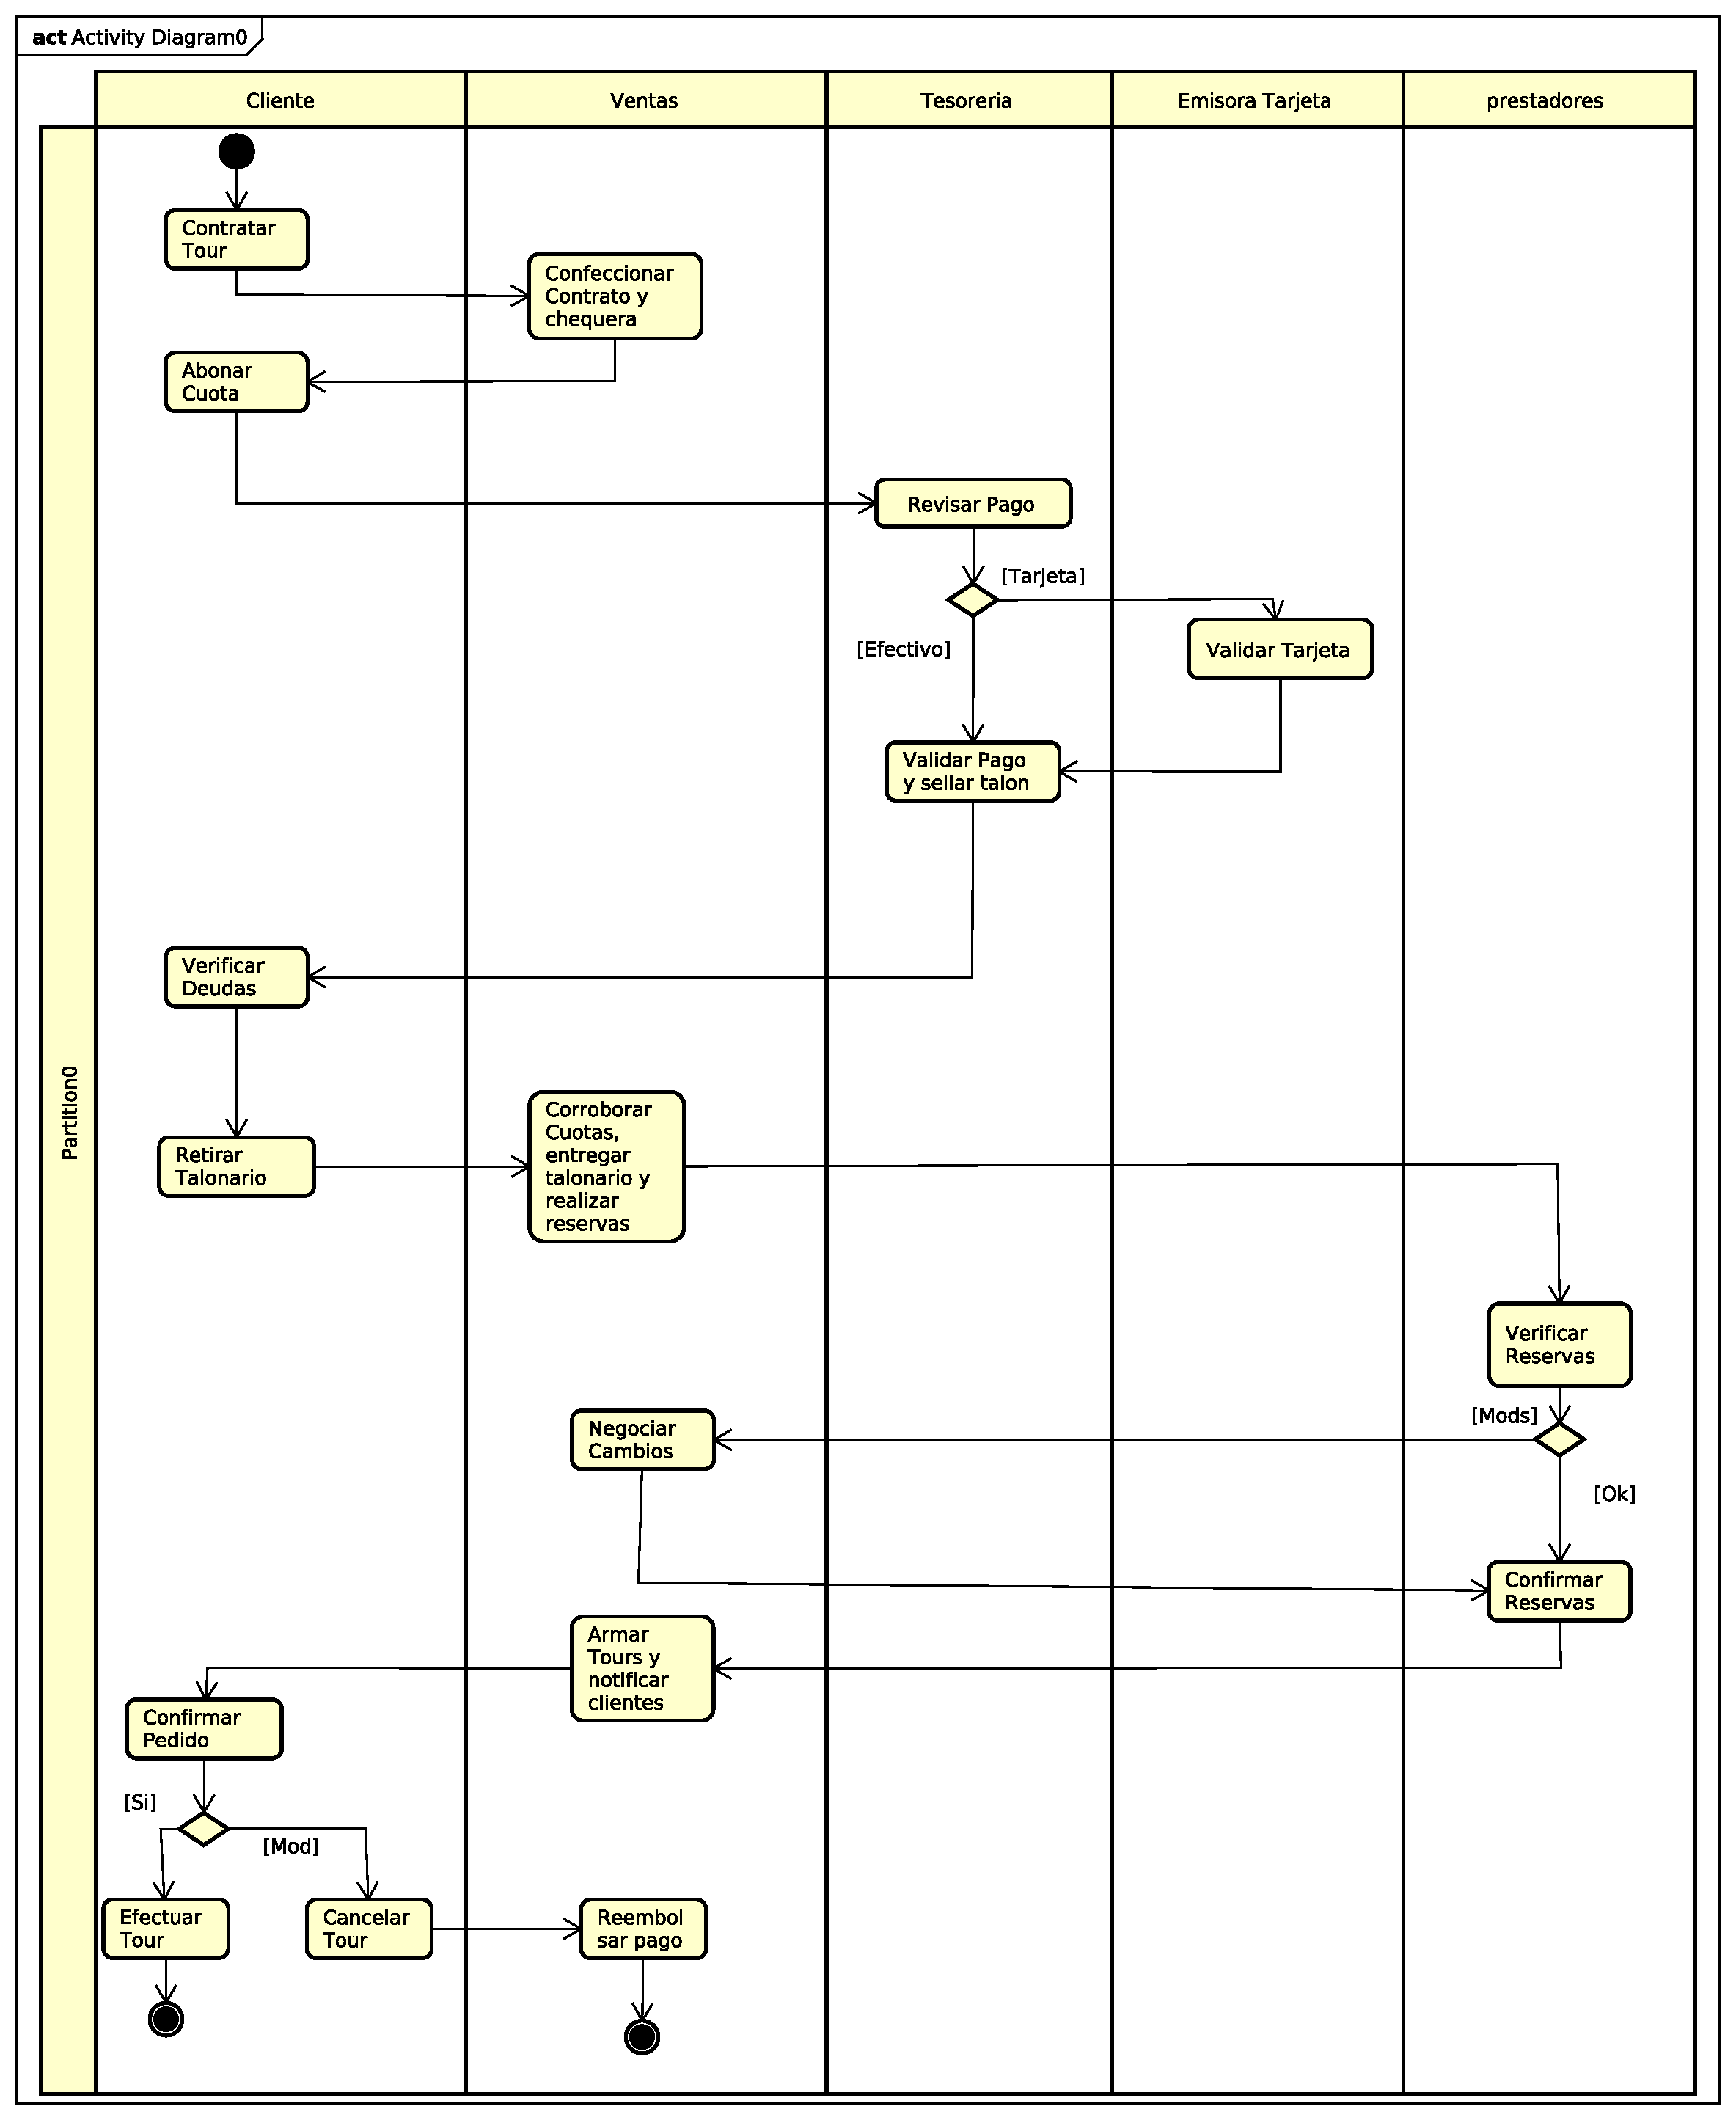
\includegraphics[scale=0.45]{images/Activity_Diagram0.pdf}

\newpage
\section{Modelo de Casos de Uso}
	\subsection{Identificación de Actores}
		\begin{itemize}
			\item \textbf{Cliente:} Es la persona que efectúa la contratación de un tour con la empresa.
			\item \textbf{Entidad Bancaria:} Es la entidad bancaria encargada de corroborar los pagos efectuados mediante tarjeta de crédito.
			\item \texbf{Administrador:} El encargado de mantener los clientes y los tours.
			\item \textbf{Prestadores:} Son quienes prestan los servicios incluidos en los tours.
			\item \texbf{Temporales:} Son aquellos que se ejecutan durante un lapso de tiempo para realizar una tarea específica.
		\end{itemize}

	\subsection{Identificación de Casos de Uso}
		\begin{itemize}
			\item \textbf{Contratar Tour:} Proceso por el cuál un cliente define el destino, las excursiones y el traslado. Se fijan las condiciones del servicio y se entrega una chequera de pago en caso de estar todo bien, caso contrario, se descarta el contrato.

			\item \textbf{Abonar Cuota:} Mensualmente, el cliente deberá abonar cada una de sus cuotas, en efectivo o con tarjeta de crédito previa validación de la entidad bancaria. 

			\item \textbf{Verificar Estado del Tour:} El cliente podrá verificar el estado del tour en todo momento. Esto implica darle información del estado del traslado, las reservas hoteleras, las excursiones y los pagos realizados.

			\item \textbf{Retirar Talonario:} Antes de realizar el tour, el cliente deberá retirar el talón con las órdenes de servicio correspondientes. Previamente se deberá corroborar que el cliente posea todas sus cuotas pagas mediante la chequera sellada.

			\item \textbf{Devolución de Pagos:} En el caso de que el cliente haya abonado el tour y los servicios no se encuentren disponibles, se le devolverá el importe completo si así lo requiere, previa validación del monto mediante la chequera.

			\item \textbf{Reservar Servicios:} Luego de que el cliente contrate un tour, se prodecerá a la reserva de los servicios correspondiantes al mismo.

			\item \textbf{Armar Tour:} Ante modificaciones por parte de los prestadores de servicios (cambios, demoras o anulaciones), se deberán armar los nuevos tours con la información nueva.

			\item \textbf{Notificar Novedades:} En caso de que los prestadores presente modificaciones que afecten los requerimientos del cliente, se les notificará permitiéndoles confirmar, modificar o anular las reservas.

			\item \textbf{Enviar Promociones y Ofertas:} Mensualmente, se deberá informar a los clientes habituales de las promociones y ofertas vigentes.

			\item \textbf{Mantener Cliente:} Se deberá tener actualizado el registro de clientes para conservar el contacto. Esto implica estar informado y mantener comunicación por algún medio de comunicación (fax, correo, e-mail u otros). 

			\item \textbf{Mantener Tour:} Se deberá tener actualizado el registro de los tours, para poder tener actualizadas las ofertas. Esto implica tener comunicación con los proveedores de servicios.
		\end{itemize}

\section{Modelo de Clases}
	\subsection{Diagrama de Clases}
		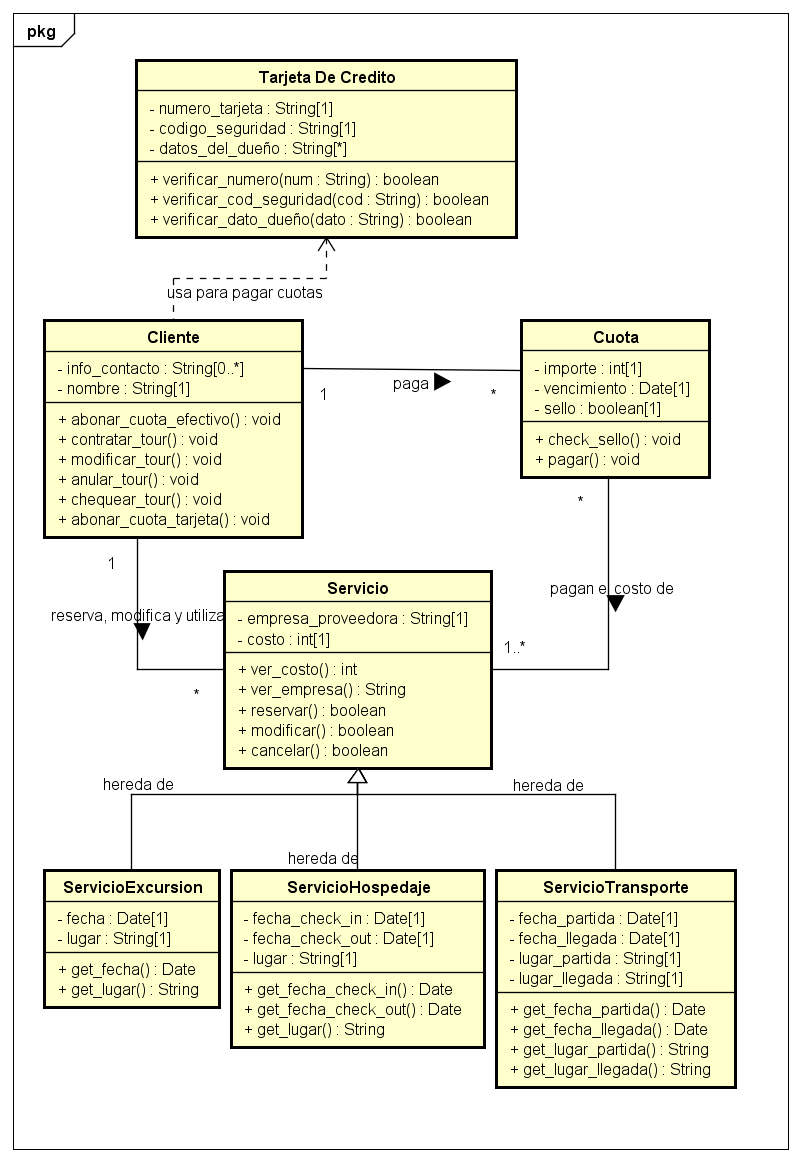
\includegraphics[scale=0.75]{diagramaDeClases.png}

\section{Diagramas de Interacción}
	\subsection{Diagrama de Secuencia}
		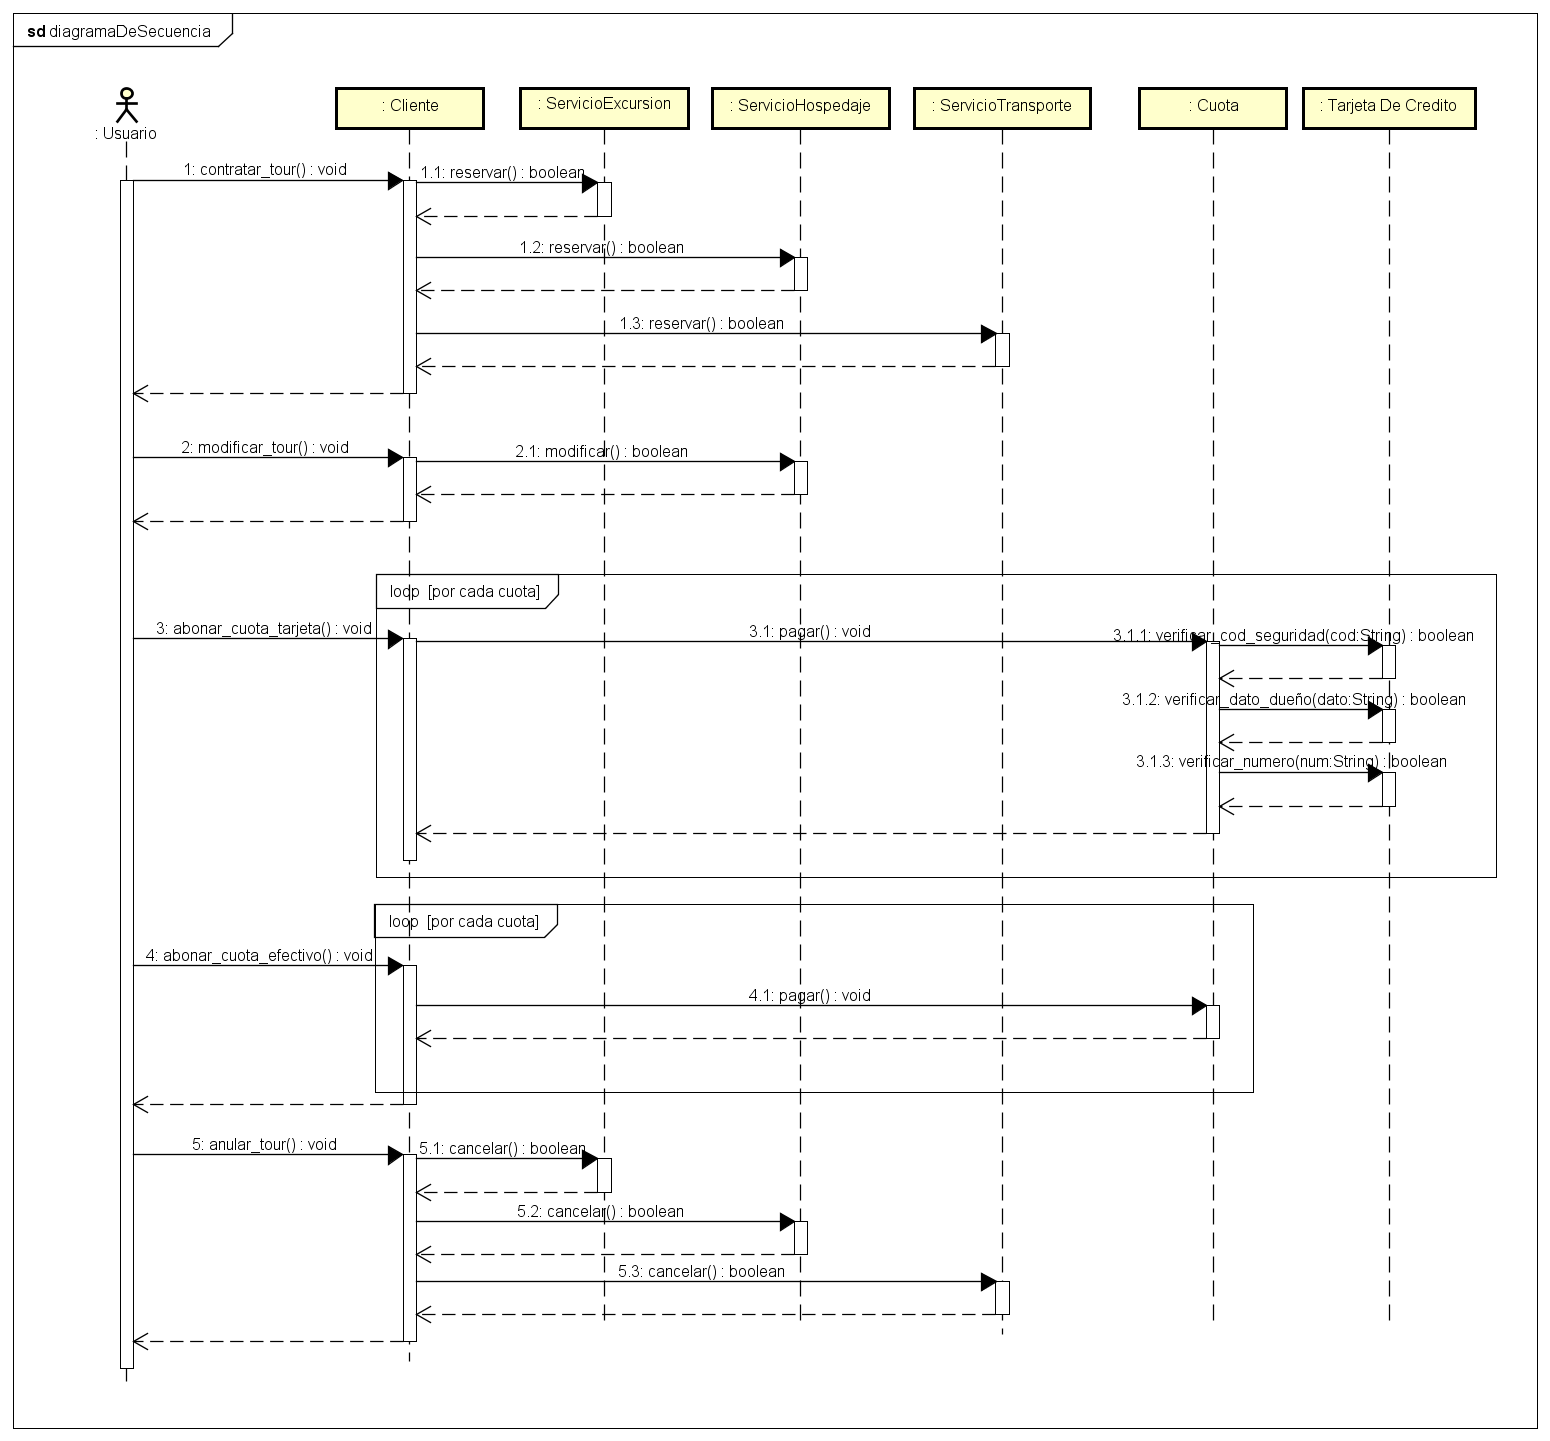
\includegraphics[scale=0.45]{diagramaDeSecuencia.png}

	\subsection{Diagrama de Colaboración}
		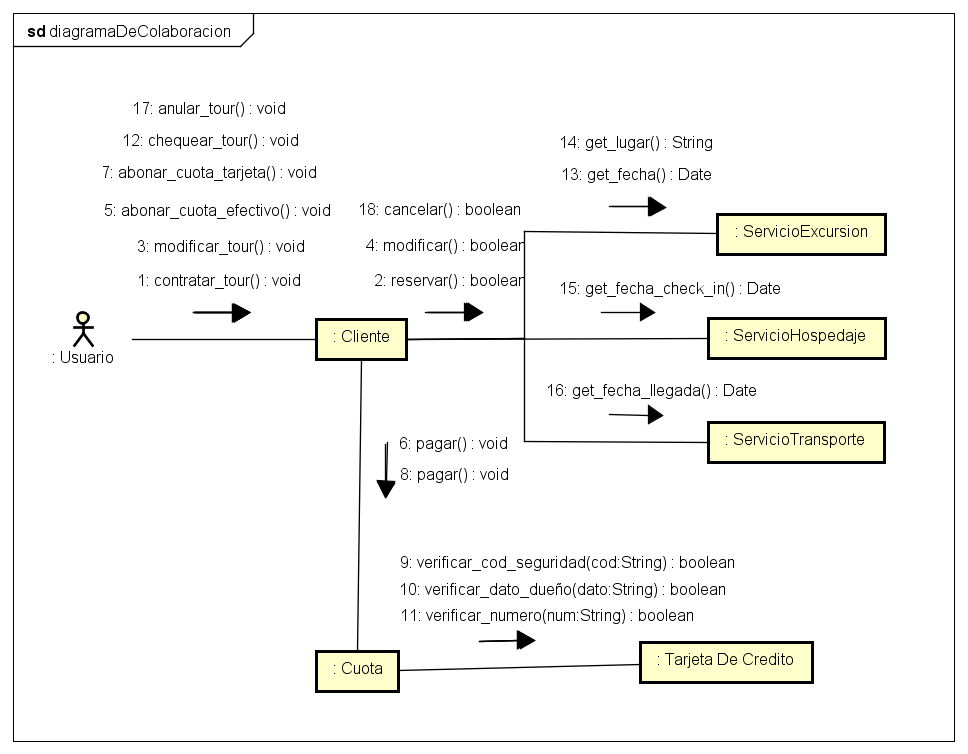
\includegraphics[scale=0.7]{diagramaDeColaboracion.png}
\end{document}